%% ****** Start of file apstemplate.tex ****** %
%%
%%
%%   This file is part of the APS files in the REVTeX 4.2 distribution.
%%   Version 4.2a of REVTeX, January, 2015
%%
%%
%%   Copyright (c) 2015 The American Physical Society.
%%
%%   See the REVTeX 4 README file for restrictions and more information.
%%
%
% This is a template for producing manuscripts for use with REVTEX 4.2
% Copy this file to another name and then work on that file.
% That way, you always have this original template file to use.
%
% Group addresses by affiliation; use superscriptaddress for long
% author lists, or if there are many overlapping affiliations.
% For Phys. Rev. appearance, change preprint to twocolumn.
% Choose pra, prb, prc, prd, pre, prl, prstab, prstper, or rmp for journal
%  Add 'draft' option to mark overfull boxes with black boxes
%  Add 'showkeys' option to make keywords appear
\documentclass[aps,prl,preprint,groupedaddress]{revtex4-2}
%\documentclass[aps,prl,preprint,superscriptaddress]{revtex4-2}
%\documentclass[aps,prl,reprint,groupedaddress]{revtex4-2}

% You should use BibTeX and apsrev.bst for references
% Choosing a journal automatically selects the correct APS
% BibTeX style file (bst file), so only uncomment the line
% below if necessary.
%\bibliographystyle{apsrev4-2}

\usepackage{graphicx}
\usepackage{amsfonts}
\usepackage{amssymb}
\usepackage{bm}
\usepackage{bbold}
\usepackage{color}
\usepackage[breaklinks]{hyperref}
\usepackage{epstopdf, epsfig}

\newcommand{\bX}{\bm X}
\newcommand{\bu}{\bm u}
\newcommand{\bF}{\bm f}
\begin{document}

% Use the \preprint command to place your local institutional report
% number in the upper righthand corner of the title page in preprint mode.
% Multiple \preprint commands are allowed.
% Use the 'preprintnumbers' class option to override journal defaults
% to display numbers if necessary
%\preprint{}

%Title of paper
\title{Steering undulatory microswimmers in a moving fluid through machine learning}
% Addresses
\newcommand{\cemef}{Ecole Nationale Sup\'erieure des Mines de Paris, PSL University, CNRS, Cemef, Sophia-Antipolis, France}
\newcommand{\inria}{Universit\'e C\^ote d'Azur, Inria, CNRS, Cemef, Sophia-Antipolis, France}

\author{Rapha\"{e}l Chesneaux} \affiliation{\cemef}
\author{La\"etitia Giraldi} \affiliation{\inria} 
\author{J\'er\'emie Bec} \affiliation{\cemef} \affiliation{\inria}

\date{\today}

\begin{abstract}
    A new model of microswimmer is introduced to investigate locomotion strategies based on the sinusoidal undulation of a slender body. These active particles are then embedded in a prescribed fluid flow in which their swimming undulations have to compete with the drifts, strains and deformations inflicted by the outer velocity field. Such an intricate situation, in which swimming and navigation are tightly bonded, is addressed using reinforcement learning. It is shown that the displacement strategy of the microswimmers can be efficiently optimized using $Q$-learning. Still, such an approach rapidly becomes rather expensive because of the highly chaotic character of the swimmers dynamics yielding a strong variability in learning efficiencies. A genetic algorithm is employed to circumvent such a pitfall.
\end{abstract}

\maketitle

\section{Introduction}
% PRESENTATION DES EQUATIONS DU MOUVEMENTS
Microorganisms such as bacteria or plankton are natural examples of self-propelled particles. They often inspire the design of artificial devices used for industrial micro-manufacturing, toxic waste disposal, targeted drug delivery or localized medical diagnostics~\cite{wu2020medical}. Recent technological developments on the use of micro-swimmers in medicine open new frontiers: those of surgery at the microscopic scale, directly inside the human body, enabling to deliver medicine and drugs in very precise places where their efficiency will be optimal. Much work was devoted to designing adequate nanorobots and studying the way they can be propelled and controlled  using an external  magnetic field~\cite{Magneticswim}, in particular for \textit{in-vivo} conditions. Many questions are still open on how these micro-swimmers optimize their displacement, and in particular how they behave in complex flows comprising obstacles, walls, or having non-Newtonian properties. This is particularly important in order to find new designs and strategies that will allow artificial swimmers to reach new regions of the human body.

Studying and optimizing the displacement of swimmers and micro-swimmers is generally addressed in two successive steps. The first consists in finding an appropriate \textit{swimming strategy} by choosing the composition, shape, or deformation that will lead to an efficient locomotion of the swimmer. The second step is to define a \textit{navigation strategy} that will allow accounting for obstacles, for fluctuations in the surrounding flow, for its geometry, with the aim to minimize the time needed or the energy used to reach a target. Studying swimming strategies at the microscopic level requires advanced tools to describe fluid-structure interactions~\cite{berti2020swimming}, to take a non-Newtonian rheology of the surrounding fluid into account~\cite{shen2011undulatory}, to model the hydrodynamics stresses due to the vicinity of walls~\cite{daddi2021hydrodynamics}. Finding an effective strategy then relies on biomimetics~\cite{borazjani2009numerical,cohen2010swimming} or on solving costly problems of optimal control~\cite{alouges2013self}. As a matter of fact, such swimming issues are most of the time addressed in situations where the surrounding flow is at rest. This is justified by the complexity and the computational costs that would be required to accurately model the intricate fluid-structure interactions occurring in a chaotic or turbulent medium. 

Regarding navigation problems, there is an increasing interest in considering complicated carrier flows. The swimming mechanisms are then, most of the time, oversimplified and one rather focuses on how to adjust macroscopic active features of the swimmers in order to optimize their long-term displacement. Under such conditions, the use of machine learning techniques has proved efficiency~\cite{cichos2020machine}. Reinforcement learning has for instance been used to address navigation in a turbulent flow and to construct strategies that allow swimmers to find optimal paths to their targets in such a chaotic and fluctuating environment~\cite{reddy2016learning,colabrese2017flow,alageshan2020machine}. Navigation problems have also been studied from different perspectives such as finding new paths in the presence of obstacles that can be modelled as a potential barrier~\cite{schneider2019optimal}. 

Here we want to address the two problems at once.  The goal of this study is to demonstrate the applicability of machine learning approaches in a mesoscopic model of swimmer, and in particular to understand if such approaches are able, not only to make the swimmer move, but also to have it at the same time navigating in a complex environment. The swimmer will consist in a simple, deformable, inextensible thin filament described by the slender-body theory, and evolving in a space-varying incompressible fluid. Among the different types of swimming, we have chosen wave locomotion which is a self-propulsion strategy that relies on the generation and propagation of waves along the swimmer. This is a relatively simple, but remarkably robust technique that builds on the interactions between the swimmer and the fluid and appear in a variety of swimming strategies observed in nature. We will study the swimmer's locomotion and navigation in a periodic cellular flow and then try to optimize it path using a $Q$-learning reinforcement algorithm.



\section{A mathematical model of microswimmer}

\subsection{Dynamics of a slender flagella}

We consider that the swimmers are elongated, flexible and inextensible. They are moreover very thin, meaning that their cross-section diameter $d$ is much smaller than their length $\ell$. This assumption allows describing their interactions with the fluid in terms of the slender-body theory~\cite{lindner2015elastic}. The swimmer is moreover embedded in an incompressible fluid flow whose unperturbed velocity field is denoted by $\bu(\boldsymbol{x},t)$. The swimmer's conformation at time $t$ is characterized by a curve $\bX(s,t)$ parametrized by its arc-length $s\in[-\ell/2,\ell/2]$. The dynamics of the fiber is given by the Cosserat equation, so that
\begin{eqnarray}
  \sigma\,\partial_t^2\bX  &=& - \zeta\,\mathbb{R}\left[\partial_t \bX-\bu(\bX,t)\right] \nonumber\\
  && +\ \partial_s(T\partial_s \bX) - K\,\partial_s^4 \bX + \bF(s,t).
  \label{eq:vel_fib-NA}
\end{eqnarray}

The first force on the right-hand side is the force exerted by the fluid. It involves the drag coefficient $\zeta = 8\pi\nu\rho_{\rm f}/[2\log(\ell/d)-1]$ (with $\nu$ the fluid kinematic viscosity and $\rho_{\rm p}$ its density) and the local Oseen's resistance tensor $\mathbb{R} = \mathbb{1} -(1/2)\,\partial_s\bX\,\partial_s\bX^{\mathsf{T}}$. The second force in the right-hand side is the tension whose amplitude $T$ is determined by the inextensibility constraint $|\partial_s\bm X(s,t)| = 1$, valid at all time along the swimmer. The third term is the bending elasticity force which depends upon the swimmer's flexural rigidity $K$ (product of Young's modulus and inertia). The last term denoted $\bF$ is an internal force that is prescribed to account for the so-called active behaviours of the swimmer and that is responsible for its locomotion. Equation~(\ref{eq:vel_fib-NA}) is associated with the free-end boundary conditions $\partial_s^2\bX(s,t) = 0$ and $\partial_s^3\bX(s,t) = 0$ at the fiber's extremities $s=\pm\ell/2$. The tension itself satisfies a second-order differential equation obtained by imposing $\partial_t |\partial_s\bX|^2=0$ with the boundary conditions $T(s,t) = 0$ at $s=\pm\ell/2$.

In the limit of very small inertia, that is when the fiber's stopping time $\sigma/\zeta$ is much sorter than any characteristic time associated to the outer fluid velocity field $\bu$, the dynamics further simplifies. It follows the over-damped limit obtained by balancing the viscous drag to the other forces in the slender-body equation, so that
\begin{equation}
  \zeta\,\mathbb{R}\left[\partial_t \bX-\bu(\bX,t)\right] = \partial_s(T\partial_s \bX) - K\,\partial_s^4 \bX + \bF(s,t).
  \label{eq:vel_fib}
\end{equation}
We focus on this equation in the sequel.
The problem depends on several non-dimensional parameters that can be there identified. A first parameter is given by the ratio $\ell/L_{\rm f}$ between the fiber's length $\ell$ and the spatial scale characteristic $L_{\rm f}$ of the fluid flow. Another parameter is ${K}/({\zeta\,L_{\rm f}^{3}\,U})$ where $U$ is the order of magnitude of the fluid velocity. It measures the fiber's flexibility. The smaller it is, the more deformable is the fiber when it is subject to a compression or a shear by the flow. These two parameters are fixed for the rest of the study with representative values. We next turn to the undulatory models used to prescribe the force $\bF$.


\subsection{Model for undulatory locomotion}

\subsubsection{Helicoidal swimming}

In order to better understand how to choose the force of locomotion, let us start with considering the case where there is no flow ($\bm u = 0$). We want to find under which conditions there exists a solution of (\ref{eq:vel_fib}) corresponding to the propagation of a wave along the fiber. We first choose this wave so that it has the shape of a circular helix and is associated with a displacement with a speed $V$ along the axis of the helix. By placing ourselves in the reference frame $(\hat{x},\hat{y},\hat{z})$ where the axis of the helix is along $\hat{z}$, we are looking for a solution which, far from the edges, would take the form
\begin{eqnarray}
  \bm X(s,t) = \left[ \begin{array}{c} R\,\cos(\nu\,s-\omega\,t) \\ \varepsilon R\,\sin(\nu\,s-\omega\,t)\\  V\,t+\tau\,s\end{array}\right] &\ \mbox{where}& \ R^2\nu^2+\tau^2 = 1\ \ \nonumber\\ &\mbox{and}& \ \varepsilon = \pm 1 ,
  \label{eq:helice}
\end{eqnarray}
where $R$ is the radius of the helix, $\tau\in[-1,1]$ its torsion and $\varepsilon$ its chirality. The curvature is constant, equal to $R\,\nu^2$, and the last condition corresponds to imposing the inextensibility of the fiber. It should be noted that this solution is not compatible with the boundary conditions satisfied by the solutions of (\ref{eq:vel_fib}). For now, it doesn't matter as we are looking for solutions taking the above form far enough from the ends of the fiber. By injecting~(\ref{eq:helice}) into the dynamical equation (\ref{eq:vel_fib}), we get
\begin{eqnarray}
  f_{\hat{x}} &=& K\,\nu^4 R\,\cos(\nu\,s-\omega\,t) \nonumber\\
  &&+ \zeta \left[\frac{\tau\,\nu}{2}V+\left(1-\frac{R^2\nu^2}{2}\right) \omega\right]R\,\sin(\nu\,s-\omega\,t), \label{eq:fxtmp}\\
  f_{\hat{y}}&=& -\zeta \left[\frac{\tau\,\nu}{2}V+\left(1-\frac{R^2\nu^2}{2}\right) \omega\right]\varepsilon R\, \cos(\nu\,s-\omega\,t) \nonumber\\
  &&+K\,\nu^4 \varepsilon R\,\sin(\nu\,s-\omega\,t), \label{eq:fytmp}\\
   f_{\hat{z}} &=& \zeta\left(1-\frac{\tau^2}{2}\right)V +\zeta\,\frac{\tau\,\nu}{2}\,R^2\omega \label{eq:fztmp},
 \end{eqnarray}
The inextensibility condition $|\partial_s \bm X |^2 = 1$ is satisfied by the solution (\ref{eq:helice}) at every moment of time. This explains why the terms involving the tension do not appear in the above system.

In the case where $\zeta\neq0$ and where we impose that the force is not a global source of momentum for the swimmer, namely $\int\bm f \mathrm{d}s = 0$, we get from (\ref{eq:fxtmp}-\ref{eq:fztmp}) that $\nu$ has to be chosen as a multiple of $(2\pi/\ell)$ and that $f_{\hat{z}} = 0$. With this choice, the displacement speed is written as a function of the parameters of the locomotion force as
\begin{equation}
  V = -\frac{\omega\,R^2\nu\,\tau}{2-\tau^2} = -\frac{\omega}{\nu} \, \frac{\tau\,(1-\tau^2)}{2-\tau^2}.
\end{equation}
The swimming speed $V$ in the absence of fluid flow is thus proportional to the phase velocity $\omega/\nu$ with a constant that solely depends upon the helix torsion $\tau$ imposed by the locomotion forcing.

For our study, we decided to characterize the force amplitude by a non-dimensional parameter $\alpha$, so that we have for $\bF$ 
\begin{eqnarray}
  f_{\hat{x}} &=& B\cos(\nu\,s-\omega\,t) + A\sin(\nu\,s-\omega\,t), \label{eq:fxfinal}\\
  f_{\hat{y}}&=& -A\cos(\nu\,s-\omega\,t)+B\sin(\nu\,s-\omega\,t), \label{eq:fyfinal}\\
   f_{\hat{z}} &=& 0 \label{eq:fzfinal},
 \end{eqnarray}
Where $A = \alpha\,\zeta\,\omega/\nu$ and $B=K\nu^4\,R$
This solution therefore makes it possible to construct an adequate force for the locomotion of the fiber in a given direction $\bm p$. It is parameterized by the wave number $\nu$, the frequency $\omega$ and the dimensionless parameter $\alpha$. Its expression is of the form $\bm f=[\bm m,\bm n,\bm p]\, [f_{\hat{x}}, f_{\hat{y}},0]^{\mathsf{T}} $ where $\bm m$ and $\bm n$ are two orthogonal unit vectors, both orthogonal to $\bm p$, the expressions of $f_{\hat{x}}$ and $f_{\hat{y}}$ being given by (\ref{eq:fxfinal}) and (\ref{eq:fyfinal}).

\subsubsection{Planar undulatory swimming}
Another choice of force that we have studied consists in propagating a sinusoidal plane wave along the fiber. In that case, the force is chosen to be 
\begin{equation}
    \bF(s,t) = A\,\cos(\nu\,s-\omega\,t)\,\bm p
    \label{eq:sinusoidal_force}
\end{equation}
where $\bm p$ is a unit vector in a direction orthogonal to that in which the swimmer is expected to move. Like in the helicoidal case, we write the forcing amplitude as $A = \alpha\,\zeta\,\omega/\nu$ where $\alpha$ is a dimensionless parameter that controls its strength. Furthermore we have the same constraint on $\nu$ coming from the global conservation of momentum.

\begin{figure}[ht]
  \centerline{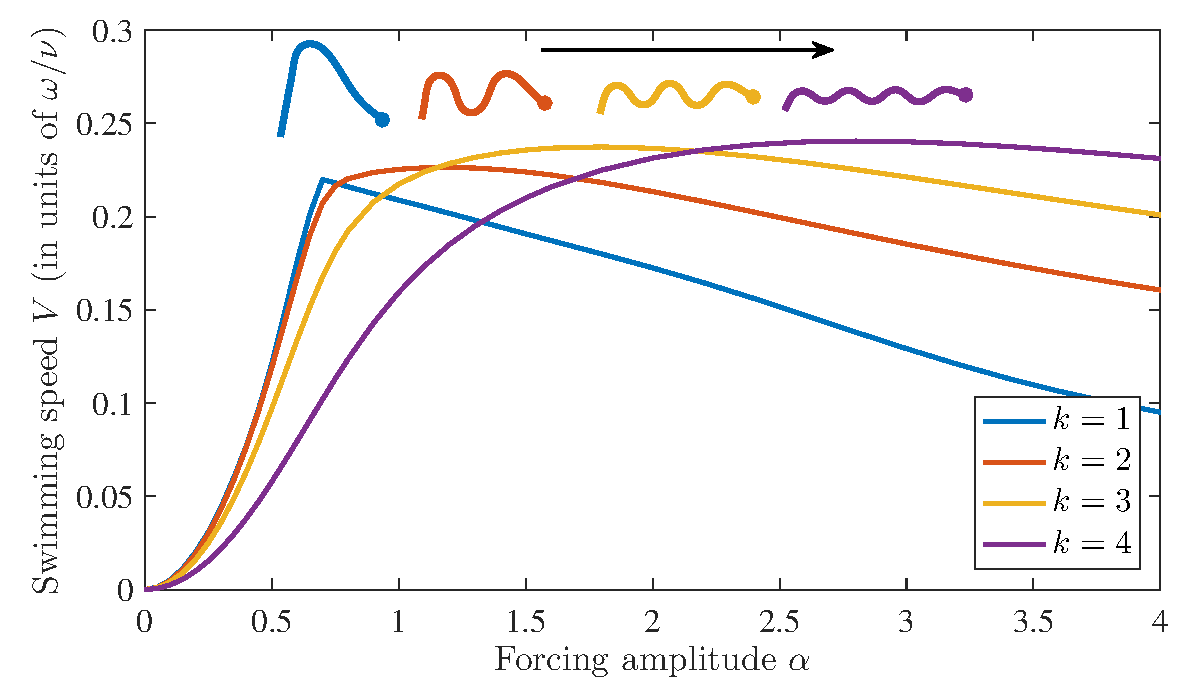
\includegraphics[width=\columnwidth]{swimming_speed_nofluid}}
  \caption{\label{fig:swimming_speed_nofluid} Swimming speed $V$ as a function of the forcing amplitude parameter $\alpha$ for different wavenumbers $k$ with $\nu = 2\,\pi\,k/\ell$ and a fixed value of the phase velocity $\omega/\nu$.}
\end{figure}
Contrarily to the helicoidal case, there is now no straightforward analytic relation between the swimming speed $V$ and the force amplitude. This is due to the intricate role played by inextensibility and tension that prevents from obtaining an explicit solution for the fiber's conformation $\bX$. We thus have recourse to numerics in order to study the dependence of $V$ upon the forcing parameter $\alpha$. We expect from dimensional considerations on space and time scales that the swimming speed will again be proportional to the phase velocity $\omega/\nu$. This is confirmed by numerics. The dependence upon the amplitude parameter $\alpha$ and the wavenumber $k$ is shown for a fixed value of $\omega/\nu$ in Fig.~\ref{fig:swimming_speed_nofluid}. The swimming speed has a maximum (of the order of $0.2\,\omega/\nu$) that slowly increases as a function of $k$ and shifts toward larger values of $\alpha$. Our results suggests that achieving a given swimming speed becomes more energetic when the wave number of the undulation increases.

These numerical results were obtained by integrating the over-damped Cosserat equation~(\ref{eq:vel_fib}) for isolated fibers in a fluid flow at rest. We use the second-order finite-difference scheme of~\cite{tornberg2004simulating} with $N=201$ gridpoints along the fiber's arclength. The inextensibility constraint is achieved by a penalization method. Time marching uses a second-order semi-implicit Adams-Bashforth method with time step $\delta t = 5\times10^{-4}$).

\

We hereafter focus on this planar undulatory locomotion model with a wavenumber $k=2$ and get interested in the following problem: we want the swimmer to swim as fast as possible in the $x>0$ direction. This amounts to choose $\bm p$ perpendicular to $\bm e_x$. It is interesting to point out the symmetry  $x\mapsto-x$ of the force because it shows that forcing the fiber to swim in the $\bm e_x$ direction by binding an $\bm e_y$ force does not lead to a movement toward $x>0$. In fact, depending on the orientation of the fiber, it can swim toward $x>0$ or $x<0$. This will have an impact on the naive swimming technique that is described below. 

% Nage dans un écoulement
\section{Swimming and navigating in a cellular flow}
From now on, we focus on the case of planar undulatory motility and consider that the swimmer is embedded is a two-dimensional cellular flow. More specifically, we choose to write the fluid velocity as $\bm u = (-\partial_y\Psi,\partial_x\Psi)$ with the stream function taking the simple periodic form $\Psi(x,t) = (L\,U/\pi)\,\cos(\pi\,x/L)\,\cos(\pi\,y/L)$. The spatial domain is hence covered by a tile of cells mimicking eddies. Their size $L$ is chosen of the same order of magnitude as the fiber length $\ell$. The velocity field has an amplitude $U$ to be compared to the swimming velocity $V$ introduced in previous section. Such a two-dimensional flow is a stationary solution of the incompressible Euler equations and is used to model the convection cells present in steady Rayleigh--B\'enard convection. It is often employed to study the effects of fluid shear and rotation on transport and mixing. It moreover has the convenience of being easily reproducible by experiments~\cite{rothstein1999persistent}. Even if the motion of tracers in such a flow is non-chaotic, the swimmer's dynamics is. Our aim is here to study how a swimming fiber embedded in such a cellular flow is able to move depending on various strategies. We first propose a naive strategy whose efficiency is then compared to that obtained from machine learning.

\subsection{A naive strategy}

Our aim is to maximize the swimmer's displacement toward the $x>0$ direction. When using the basic swimming, that is to say always binding the fiber to swim with the force (\ref{eq:sinusoidal_force}) constantly applied along the direction $\bm p = \bm e_y$, one obtains a completely chaotic motion. The fiber changes direction randomly: As illustrated in Fig.~\ref{fig:displ_nostrategy}, when arriving in a new cell, either the swimmer passes through the cell, or its orientation is reversed and it leaves in the opposite direction. Consequently, the swimmer performs a random walk on long timescales. The average displacement of the fiber's center of mass is therefore zero.

\begin{figure}[ht]
  \centerline{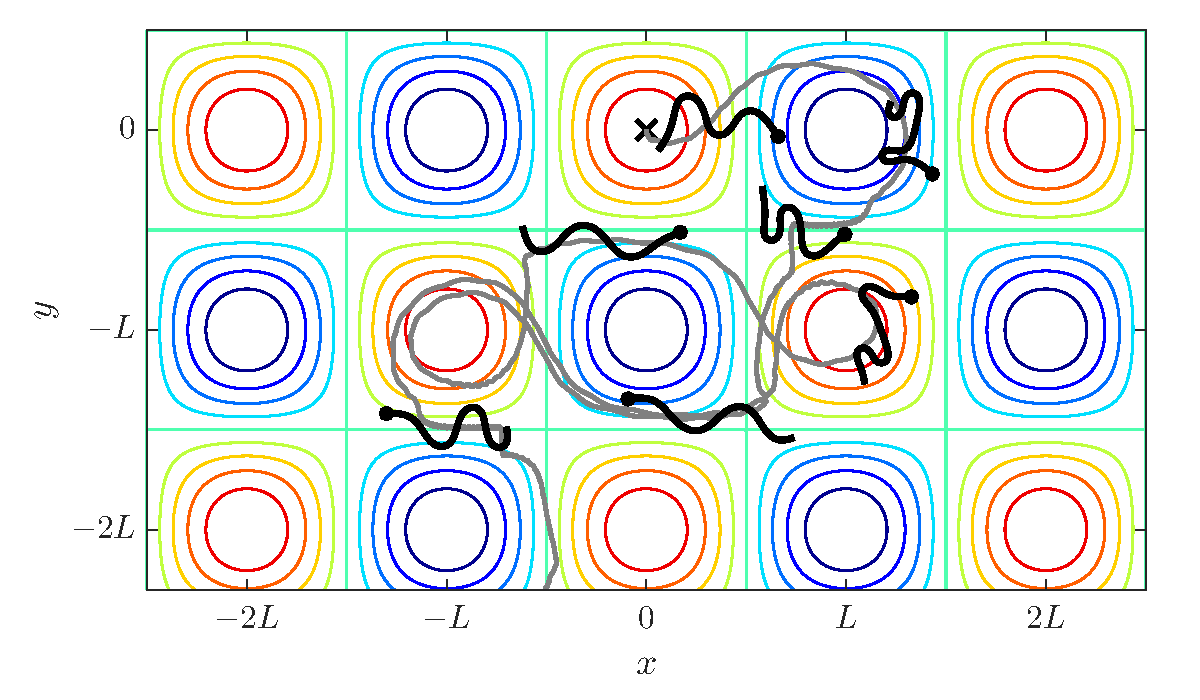
\includegraphics[width=\columnwidth]{displ_nostrategy}}
  \caption{\label{fig:displ_nostrategy} Case of a swimmer that continuously swims in the horizontal direction, with no specific strategy. It is initially released from the origin (shown as a cross) and the trajectory of its center of mass is shown as a gray curve. Several configuration are shown at different times. The colored background shows the fluid streamlines with, in red, the clockwise vortices and, in blue, those turning in the opposite direction.}
\end{figure}

A strategy allowing the swimmer to move in the $x>0$ direction is what we call the \textit{naive strategy}. It is simple: If the swimmer has the proper orientation, that is when the abscissa difference between its head and its center of mass is positive, the sinusoidal force (\ref{eq:sinusoidal_force}) is applied in the direction $\bm p = \bm e_y$. If the fiber is wrongly aligned and faces the $x<0$ direction, then we don't impose any force and the locomotion is stopped. This is a simple strategy that can be easily understood and induces a positive drift by breaking the symmetry $x\mapsto-x$. The results obtain with such a swimming are better than in the absence of any strategy and we get a positive average displacement. 

\begin{figure}[ht]
  \centerline{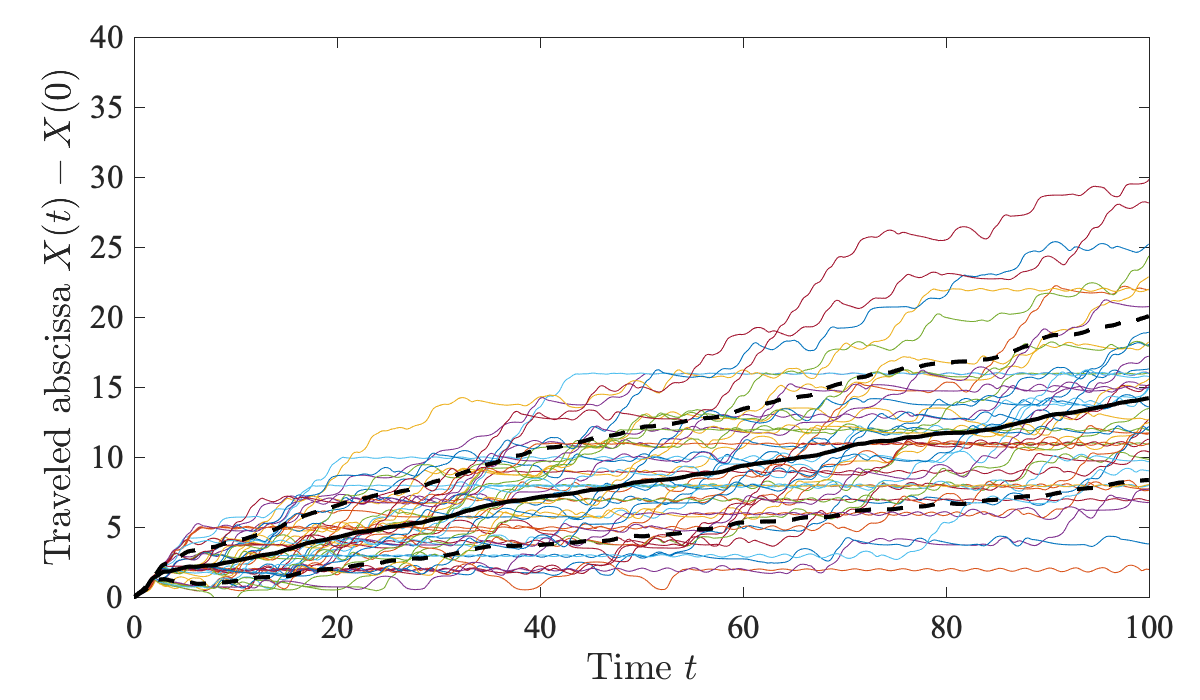
\includegraphics[width=\columnwidth]{travel_naive_diffreal}}
  \caption{\label{fig:travel_naive_diffreal} Horizontal displacement of swimmers following the naive strategy, together with the average shown as a bold solid line, and the interval defined by the standard error shown as dashed lines. Time is here expressed in units of $(2\,\pi\,\omega)^{-1}$ and displacement in units of the cell size $L$.}
\end{figure}
We simulated around 50 fibers with different initial conditions. Each fiber starts at the center of a cell, with a completely unfold configuration and with a random angle with the horizontal, chosen between $-{\pi}/{2}$ and ${\pi}/{2}$. As we can see in Fig.~\ref{fig:travel_naive_diffreal} the naive strategy has a positive average displacement but we observe that the distribution of swimmers significantly spreads with time. The standard deviation of the displacement increases with time and, in some cases, the displacement stays at an approximately constant value during rather long times, showing that the swimmers can get trapped in a cell and stop progressing to positive $x$.  To improve our results and allow for a faster displacement, we next rely on machine-learning techniques and implement a $Q$-learning method.


% OPTIMIZATION PART
\subsection{An optimal strategy using $Q$-learning}
We use the classical $Q$-learning algorithm with a set of discrete states $\mathcal{S}$ and discrete actions $\mathcal{A}$. The policy is described by the $Q$-table, which assigns at time $t$ to each couple $(s,a)\in \mathcal{S}\times \mathcal{A}$ a mark $Q_t(s,a)$. The action $a_t$ taken at time $t$ is such that it maximizes $Q_t(s_t,\cdot)$.

We define the swimmer's state as a combination of 3 features. The first property is the horizontal component of the fluid velocity at the fiber's head $u_{\rm h} = \bm e_x\cdot \bu(\bX(0,t),t)$. We use a parameter $u_0$ and distinguish between three cases, $u_{\rm h}<-u_0$, $u_{\rm h}>u_0$, and $|u_{\rm h}|<u_0$, which correspond to having a headwind, a tailwind, or no significant wind caused by the fluid flow. The second state parameter is the swimmer orientation, either towards positive $x$ or towards negative $x$. It is defined as the sign of the abscissa difference between the fiber's head and its center of mass. The last state parameter accounts for the presence or not of a loop along the fiber. This last condition comes from observations of the fiber's swimming simulations where the buckling of the swimmer's body sometimes leads to a dead end, the fiber been locked in a given cell. All these parameters define a discrete set of 12 states. Concerning the actions, we define two categories: first the direction in which the force (\ref{eq:sinusoidal_force}) is applied, either toward $\bm p = \bm e_{x}$ or toward $\bm p = \bm e_{y}$. Second the value of the amplitude parameter $\alpha$ that is chosen in $ \{0,0.5,0.75,1\}$. There is, at the end, a discrete set of 8 actions. 

The learning algorithm is based on the classical value-iteration update of the Bellman equation, namely
\begin{eqnarray}
    Q_{t+\Delta t}(s_t,a_t) &=& (1-\lambda\,\Delta t)\,Q_{t}(s_t,a_t) \nonumber\\
    &+& \lambda\,\Delta t\,\left[r_t + \gamma\,\max_a Q_{t}(s_{t+\Delta t},a) \right]\!,
    \label{eq:Qlearning}
\end{eqnarray}
where $\lambda$ denotes the learning rate, $\gamma$ the discount factor, and $r_t$ is the reward, which in our case is defined as the distance travelled in the $x$ direction by the swimmer's center of mass, namely $r_t = \bar{x}(t+\Delta t)-\bar{x}(t)$ with $\bar{x}(t) = (1/\ell) \int \bm e_x\cdot\bm X(s,t)\,\mathrm{d}s$. The time discretization of (\ref{eq:Qlearning}) involves a time step that we choose to be $\Delta t = 200\,\delta t$. The learning rate is fixed to $\lambda = 0.05$, approximately corresponding to the inverse of the time needed by the swimmer to travel across two cells. Similarly, the discount factor is chosen such that the discount time $-\Delta t / (\log \gamma)$ corresponds to the time needed by the swimmer to traverse approximately ten cells. This weights the rewards obtained by the swimmer in the distant future, allowing our reinforcement strategy to optimize long-term displacements.

\begin{figure}[ht]
  \centerline{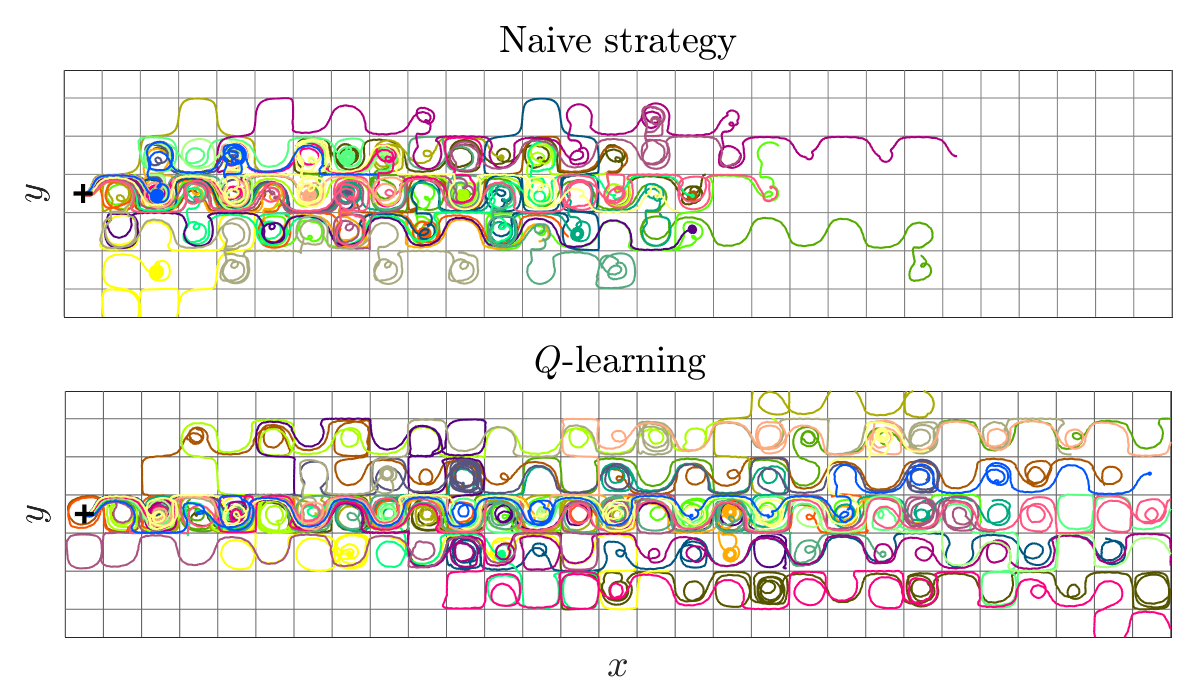
\includegraphics[width=\columnwidth]{compare_traj}}
  \caption{\label{fig:compare_traj} Typical trajectories (various colors) obtained with the naive strategy (top) and with $Q$-learning (bottom). All swimmers are released from the origin (shown as a black cross) and try to move toward $x>0$ across the various cells of our model flow.}
\end{figure}
We have simulated a set of 50 learning swimmers using for each of them different starting conditions randomly chosen. The entries of the $Q$-table are initialised to sufficiently large values, that is with optimistic premises, allowing the learning algorithm for wider explorations. Some trivially inefficient configurations have however been initially penalized. They correspond to situations where the fiber is wrongly oriented and swims against the fluid current, the later being strong enough to push the swimmer to the right. It is in that case much more efficient not to swim. We compare the performance of our $Q$-learning method with the naive strategy explained above. The $Q$-learning method rapidly display better results, as seen in Fig.~\ref{fig:compare_traj}. In the naive strategy, some fibers get locked in a cell and can not escape from it. This due to the deformation of the fiber that can buckle the swimmer's body. We can also observe that the $Q$-learning method, in addition to locking less fiber in cells, allow them to go further and to progress further to the right.


\begin{figure}[ht]
  \centerline{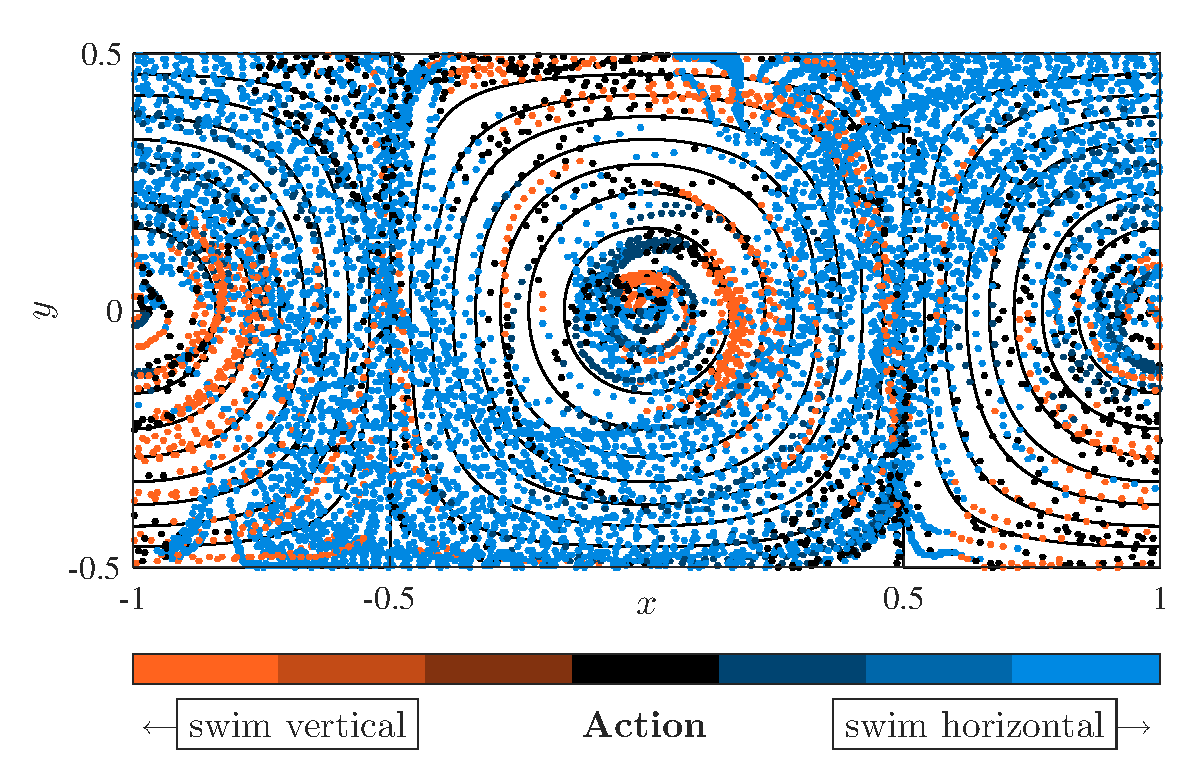
\includegraphics[width=\columnwidth]{traj_centerofmass}}
  \caption{\label{fig:traj_centerofmass} Typical trajectory of the swimmer's center of mass obtained after learning. The positions have been here folded to account for periodicity. The colors correspond to the different actions taken by the swimmer, ranging from red (swimming with $\alpha = 1$ in the $y$ direction) to blue (swimming with $\alpha = 1$ in the $x$ direction).}
\end{figure}
$Q$-learning improves the naive strategy by giving a different path to the swimmers. With this method, the fiber takes advantage of the flow by going trough high positive horizontal fluid velocity area, passing alternately through the top of a cell and through the bottom. Such a ``surfing'' is evidenced from Fig.~\ref{fig:traj_centerofmass} that shows the typical trajectory of a swimmer after it has learnt an optimal strategy. The color code display the various actions that are performed by the swimmer. When surfing on an optimal path, the fiber maximizes its swim in the $x$ direction. Conversely, when it get traps in the center of a cell or in a region of counterflow (\textit{e.g.} top of the center cell), it either stops swimming or initiate a vertical displacement.

\begin{figure}[ht]
  \centerline{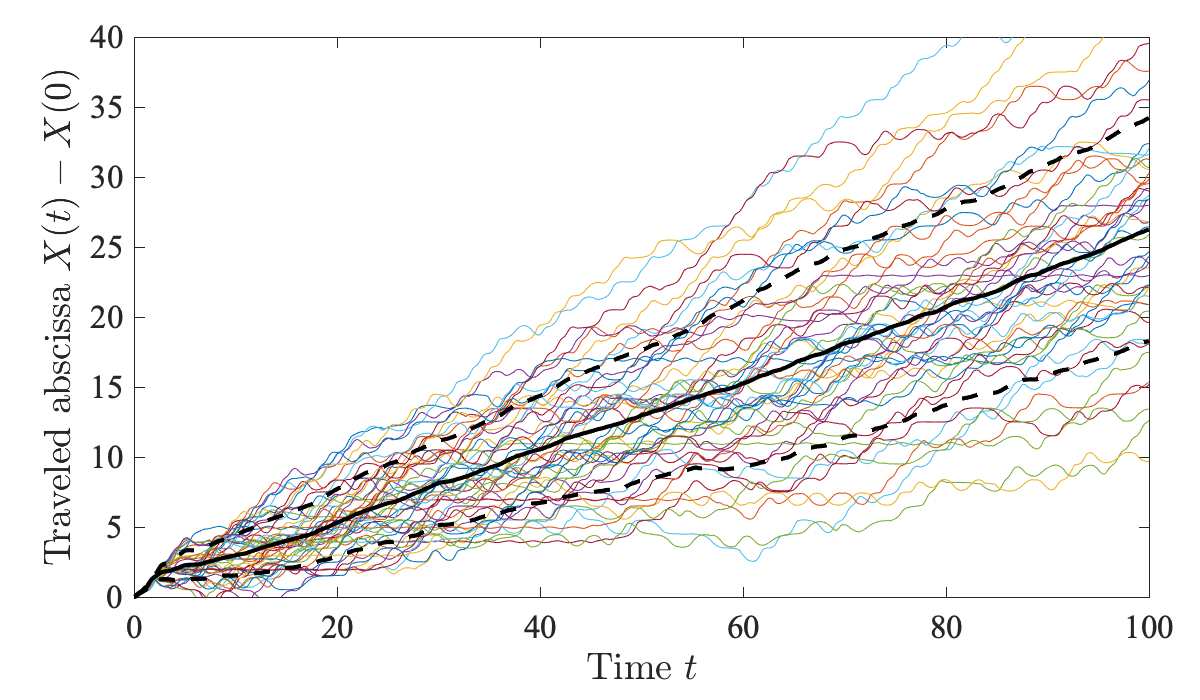
\includegraphics[width=\columnwidth]{travel_learn_diffreal}}
  \caption{\label{fig:travel_learn_diffreal} Horizontal displacement for different realizations of  learning, together with the average shown as a bold solid line, and the interval defined by the standard error shown as dashed lines.}
\end{figure}
Even if performance is significantly improved, we find that, as in the case of the naive swimmer, there is a rather strong variability in the displacement efficiency. This is evidenced from Fig.~\ref{fig:travel_learn_diffreal} that shows how a set of 50 trajectories spreads while it learns. Even if the average displacement outperforms by almost a factor 2 that obtained with the naive strategy in the same fluid flow (compare to Fig.~\ref{fig:travel_learn_diffreal}), one observes that there is still a very strong variability among the various realizations. A large number of trajectories are very far from the average. Some, maybe lucky, perform much better. Others spend a very long time trapped in a cell (some of these events are visible in the bottom panel of Fig.~\ref{fig:compare_traj}). When trapped, they possibly forget a large part of the training they acquired before. Such a variability originates from the chaotic behavior of the fibers dynamics and is responsible for also a strong variability in the learning process.



\subsection{Combining reinforcement learning with a genetic algorithm}

To correct this problem of convergence, we decided to use a genetic algorithm for our Q-learning. Indeed, we put several fibers at competition during a time $T$ and at the end we compare the progression of each fiber and find the fastest one. Then the matrix Q of this fiber is shared with the other fibers and then a run is started again during a time T with random initial conditions for each fiber. This algorithm is called genetic algorithm because we only keep the learning part of the strongest fiber, as this is the case in nature.

\begin{figure}[ht]
  \centerline{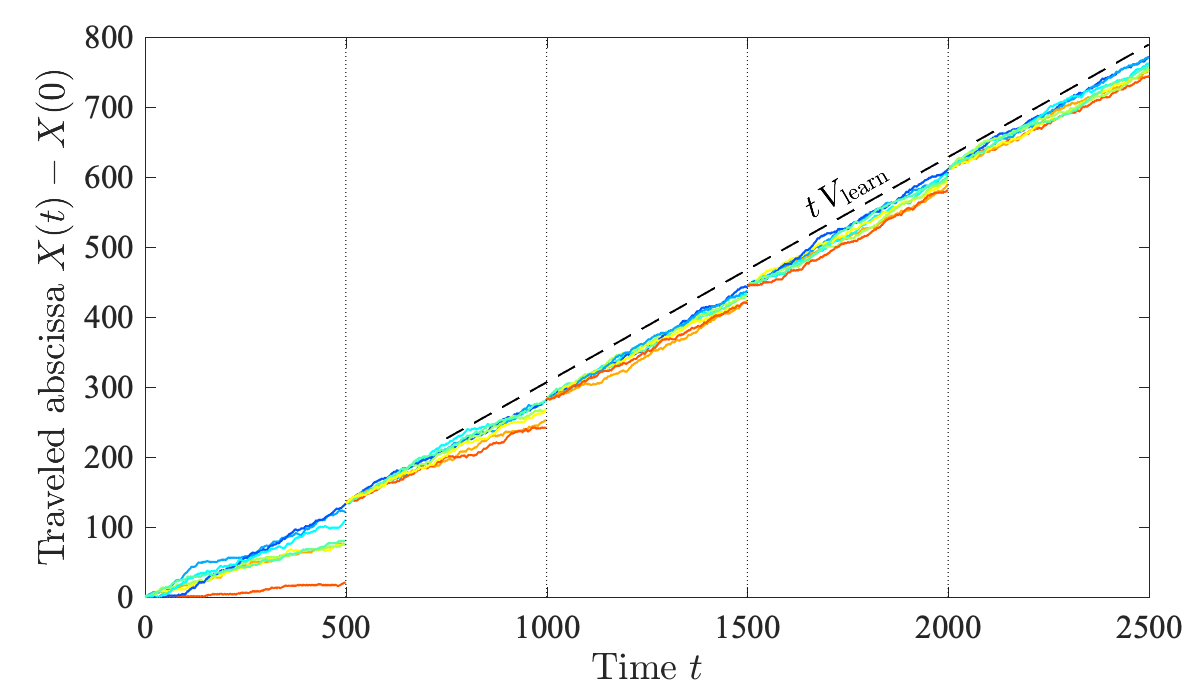
\includegraphics[width=\columnwidth]{genetic_learning}}
  \caption{\label{fig:genetic_learning} Implementation of the genetic algorithm here applied to five generations and a population of eight individuals. The horizontal displacement of individuals is periodically evaluated (at times shown as vertical dotted lines) and only the strategy developed by the best candidate (blue curve) is retained and imposed to the next generation. Swimmers position are then reinitialised at the center of a cell with a random orientation. Such an algorithm accelerates the convergence to an asymptotic swimming speed (represented as a black dashed line). }
\end{figure}

This genetic algorithm require more computing power but it increases the reproducibility and the convergence of learning towards an optimal swimming strategy. In fact, as the learning takes place, there is a convergence towards a single value of the average speed of movement of the fibers. In fact, as shown in Fig.~\ref{fig:genetic_learning}, as the various runs are carried out, we note the gradual disappearance of the fibers very far from the average path obtained with the previous method. The dispersion of the results decreases during the different runs. This highlights the implementation of a strategy during learning that allows to obtain regular results.

The simulation resulting in Fig.~\ref{fig:genetic_learning} was carried out for a fixed value of the amplitude of the flow $U$. This is why, in order to demonstrate the performance of learning using genetic algorithm, we carried out simulation by varying this value $U$ by the amplitude of the flow. This allows us to underline the dependence of the efficiency of learning on the amplitude of the flow. We can see in Fig.~\ref{fig:vel_VarU} that for all the values of $U$, Q-learning is more efficient than the naive strategy. However, this improvement is most efficient when the $\frac{U}{V_{\rm swim}}$ ratio ($V_{\rm swim}$ corresponds to the velocity of the fiber without flow ) is equal to 1. In fact, in this case, the influence of the fluid makes it possible for swimming strategy to have an impact . In the case where $ \frac{U}{V_{\rm swim}}<1$, the fluid has no impact on the swim, a straight swim is most effective. Finally in the case $ \frac{U}{V_{\rm swim}}>1$, it is the fluid which is the most important and the choice of the strategy does not matter (the fiber undergoes the flow).



\begin{figure}[ht]
  \centerline{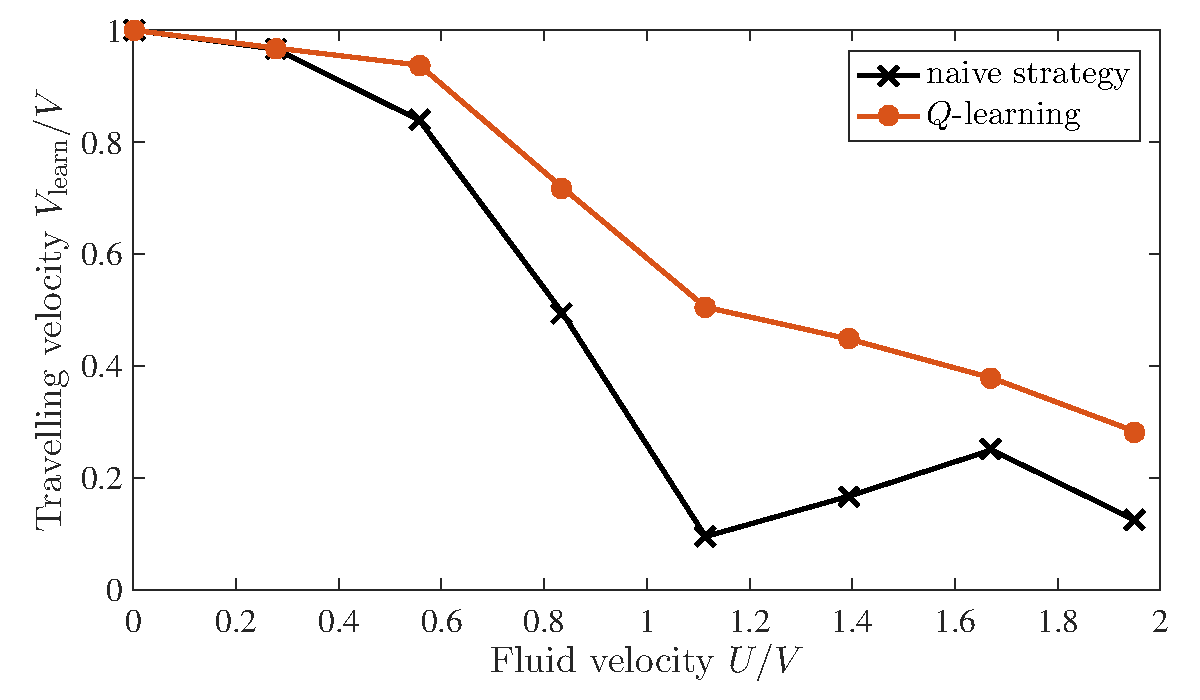
\includegraphics[width=\columnwidth]{vel_varU}}
  \caption{\label{fig:vel_VarU} Asymptotic velocity of the swimmers (here normalized by the swimming speed $V_{\rm swim}$ in the absence of fluid flow), as a function of the fluid flow amplitude $U$, with both the average value obtained with the naive strategy and the optimal value obtained with $Q$-learning, as labeled. }
\end{figure}

For the naive strategy, we can see that there is a variation of the curve at the value 1 where the average speed increases with the ratio. This is due to the fact that when $ \frac{U}{V_{\rm swim}}=1$, the fiber can be trapped in a cell when the fluid speed and the swimming are equal, the fiber going to $x>0$. That is not the case when $ \frac{U}{V_{\rm swim}}>1$ because the fluid wins and take the fiber in a more favorable position.
Finally, we have shown that this learning swim results can work under different speed regimes although it can be more efficient in certain specific cases.

\section{Concluding remarks and perspectives}

To conclude, we have presented here the mathematical models to study the swim of a fiber in a 2D cell flow. We have developed a Q-learning approach to optimize the swim strategy of the fiber maximizing the velocity. We have also developed a genetic algorithm that, combined with the Q-learning, can converge to an optimize strategy with better velocity than the naive strategy. We have therefore shown the relevance of the use of Q-learning in learning to swim in cell flows.

A possible opening for future work would consist in studying the movements of a fiber, that have been previously trained, in more chaotic turbulent flows. It is indeed a possibility that would allow studying the effects of learning with the Q-learning method in a more realistic flow. In addition, the next step could also consist in making the learning method more complex with deep learning methods with neural networks. All this makes it possible to consider a vast field of study on the swimming of the microswimmers.


% If in two-column mode, this environment will change to single-column
% format so that long equations can be displayed. Use
% sparingly.
%\begin{widetext}
% put long equation here
%\end{widetext}

% figures should be put into the text as floats.
% Use the graphics or graphicx packages (distributed with LaTeX2e)
% and the \includegraphics macro defined in those packages.
% See the LaTeX Graphics Companion by Michel Goosens, Sebastian Rahtz,
% and Frank Mittelbach for instance.
%
% Here is an example of the general form of a figure:
% Fill in the caption in the braces of the \caption{} command. Put the label
% that you will use with \ref{} command in the braces of the \label{} command.
% Use the figure* environment if the figure should span across the
% entire page. There is no need to do explicit centering.

% \begin{figure}
% \includegraphics{}%
% \caption{\label{}}
% \end{figure}

% Surround figure environment with turnpage environment for landscape
% figure
% \begin{turnpage}
% \begin{figure}
% \includegraphics{}%
% \caption{\label{}}
% \end{figure}
% \end{turnpage}

% tables should appear as floats within the text
%
% Here is an example of the general form of a table:
% Fill in the caption in the braces of the \caption{} command. Put the label
% that you will use with \ref{} command in the braces of the \label{} command.
% Insert the column specifiers (l, r, c, d, etc.) in the empty braces of the
% \begin{tabular}{} command.
% The ruledtabular enviroment adds doubled rules to table and sets a
% reasonable default table settings.
% Use the table* environment to get a full-width table in two-column
% Add \usepackage{longtable} and the longtable (or longtable*}
% environment for nicely formatted long tables. Or use the the [H]
% placement option to break a long table (with less control than 
% in longtable).
% \begin{table}%[H] add [H] placement to break table across pages
% \caption{\label{}}
% \begin{ruledtabular}
% \begin{tabular}{}
% Lines of table here ending with \\
% \end{tabular}
% \end{ruledtabular}
% \end{table}

% Surround table environment with turnpage environment for landscape
% table
% \begin{turnpage}
% \begin{table}
% \caption{\label{}}
% \begin{ruledtabular}
% \begin{tabular}{}
% \end{tabular}
% \end{ruledtabular}
% \end{table}
% \end{turnpage}

% Specify following sections are appendices. Use \appendix* if there
% only one appendix.
%\appendix
%\section{}

% If you have acknowledgments, this puts in the proper section head.
%\begin{acknowledgments}
% put your acknowledgments here.
%\end{acknowledgments}

% Create the reference section using BibTeX:
\bibliography{biblio}

\end{document}
%
% ****** End of file apstemplate.tex ******
